\documentclass[a4paper,12pt]{article}

%%% Работа с русским языком
\usepackage{cmap}					% поиск в PDF
\usepackage{mathtext} 				% русские буквы в формулах
\usepackage[T2A]{fontenc}			% кодировка
\usepackage[utf8]{inputenc}			% кодировка исходного текста
\usepackage[english,russian]{babel}	% локализация и переносы
\usepackage{xcolor}
\usepackage{hyperref}
 % Цвета для гиперссылок
\definecolor{linkcolor}{HTML}{799B03} % цвет ссылок
\definecolor{urlcolor}{HTML}{799B03} % цвет гиперссылок

\hypersetup{pdfstartview=FitH,  linkcolor=linkcolor,urlcolor=urlcolor, colorlinks=true}

%%% Дополнительная работа с математикой
\usepackage{amsfonts,amssymb,amsthm,mathtools} % AMS
\usepackage{amsmath}
\usepackage{icomma} % "Умная" запятая: $0,2$ --- число, $0, 2$ --- перечисление

%% Номера формул
%\mathtoolsset{showonlyrefs=true} % Показывать номера только у тех формул, на которые есть \eqref{} в тексте.

%% Шрифты
\usepackage{euscript}	 % Шрифт Евклид
\usepackage{mathrsfs} % Красивый матшрифт

%% Свои команды
\DeclareMathOperator{\sgn}{\mathop{sgn}}

%% Перенос знаков в формулах (по Львовскому)
\newcommand*{\hm}[1]{#1\nobreak\discretionary{}
{\hbox{$\mathsurround=0pt #1$}}{}}
% графика
\usepackage{graphicx}
\graphicspath{{pictures/}}
\DeclareGraphicsExtensions{.pdf,.png,.jpg}
\author{Бурмашев Григорий, БПМИ-208}
\title{ТВиМС, дз -- 7}
\date{\today}
\begin{document}
\maketitle
\clearpage
\section*{Номер 8 [листок 5]}
По условию величины независимы и:
\[
P(X_k = 1) = P(X_k = -1) = \frac14, \; P(X_k = 0) = \frac12, \; k \in \{1 \ldots n\}
\]
Для решения воспользуемся Facts с семинара:
\begin{center}
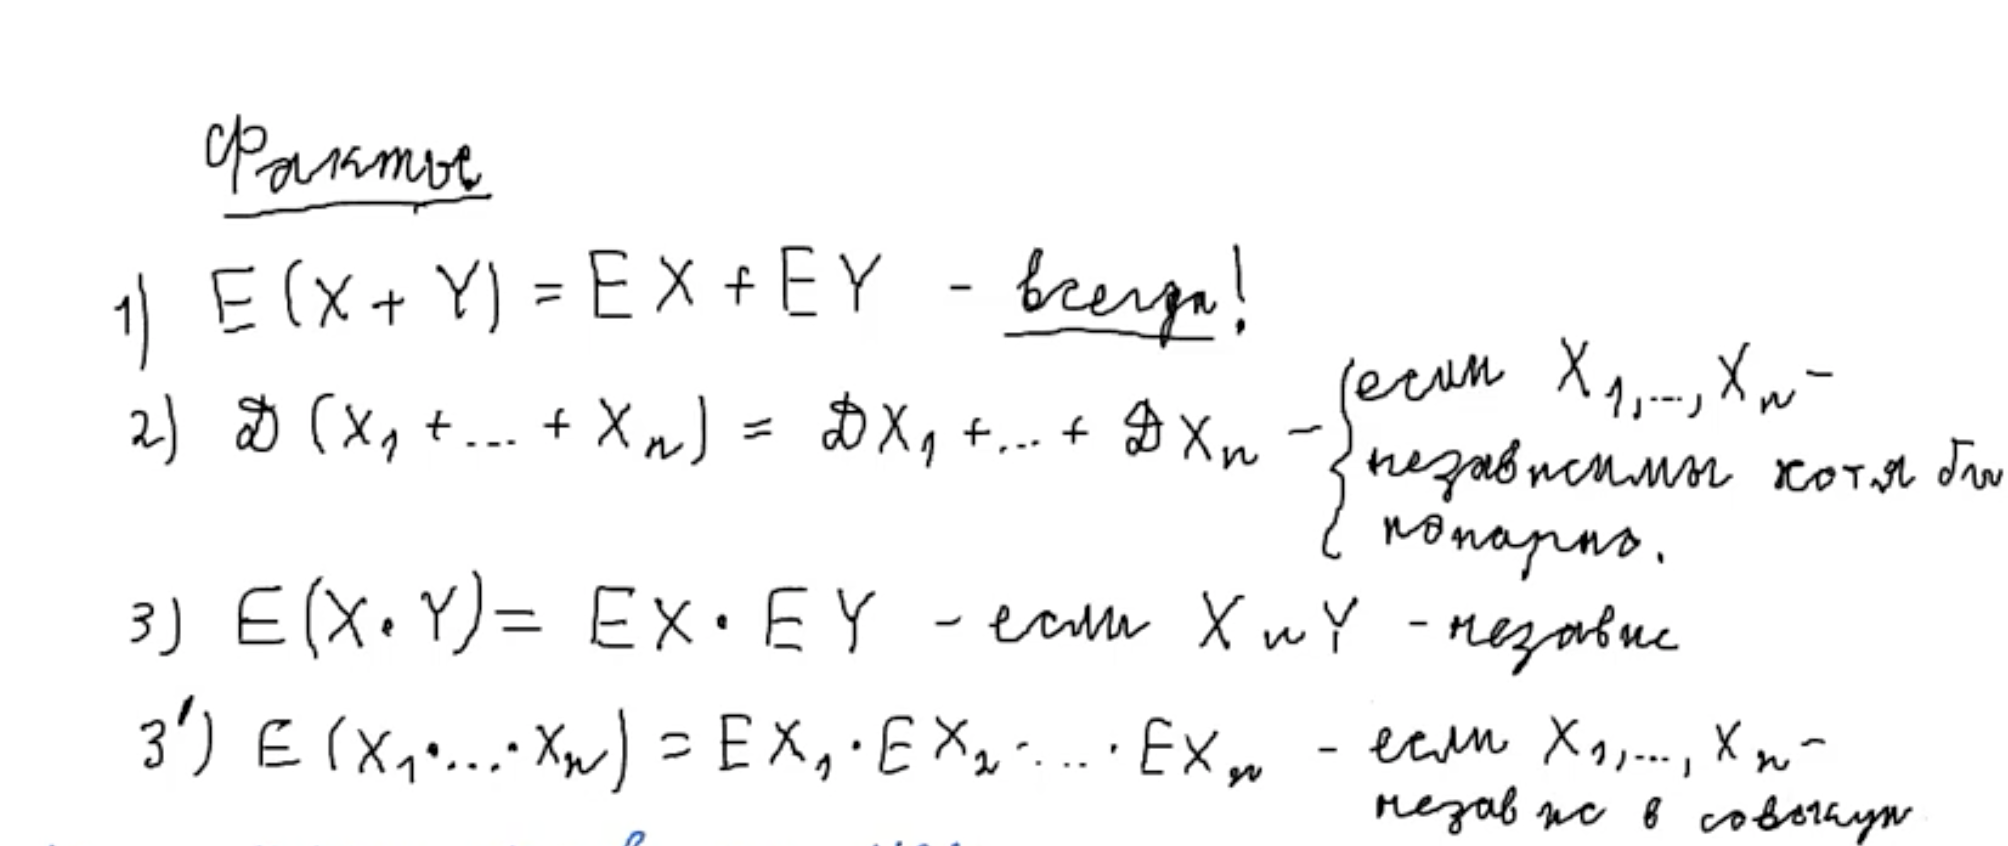
\includegraphics[scale=0.3]{1.png}
\end{center}
Тогда:
\[
\mathbb{E}S_n = \mathbb{E}(X_1 + \ldots + X_n) = \mathbb{E}X_1 + \ldots + \mathbb{E}X_n = \left(1 \cdot \frac14 - 1 \cdot \frac14 + 0 \cdot \frac12\right) \cdot n = 0
\]
\[
\mathbb{D}S_n =  \mathbb{E}S_n^2 - (\mathbb{E}S_n)^2 =  \mathbb{E}S_n^2 - 0 = \mathbb{E}S_n^2 = \left(1^2 \cdot \frac{1}{4} + (-1)^2 \cdot \frac14 + 0 \cdot \frac12 \right) \cdot n = \left(\frac24\right)n = \frac{n}{2} 
\]
\[
\mathbb{E}2^{S_n} = \mathbb{E}2^{X_1 + \ldots +X_n} = \mathbb{E}2^{X_1} \cdot \ldots \cdot \mathbb{E}2^{X_n} = \left(2^1 \cdot \frac14 + 2^{-1} \cdot \frac14 + 2^0 \cdot \frac{1}{2}\right)^n =\left( \frac{9}{8} \right)^n
\]
\begin{center}
\textbf{Ответ: } \[
\mathbb{E}S_n = 0
\]
\[
\mathbb{D}S_n = \frac{n}{2}
\]
\[
\mathbb{E}2^{S_n} = \left( \frac{9}{8} \right)^n
\]
\end{center}
\clearpage
\section*{Номер 9 [листок 5]}
Рассмотрим $i-$го человека. У него есть сосед слева и сосед справа. Все кидают кубики независимо друг от друга. Для начала проще будет сказать, когда у \textbf{обоих} соседей выпало число, которое не равно числу $i$-го человека, вероятность этого $ \frac{5}{6} \cdot \frac{5}{6} = \frac{25}{36}$, потому что нас интересует случай, когда соседу выпало любое из 6 чисел, за исключением того 1, которое выпало $i$-му. В таком случае вероятность того, что \textbf{хотя бы} у одного соседа будет число, совпадающее с нашим равна $1 - \frac{25}{36} = \frac{11}{36}$. Введем мат.ожидание для $i$-го человека (пусть $X_i$ --  индикаторная функция, которая определяет, выполняется ли нужное нам условие для $i$-го человека или нет)
\[
\mathbb{E}X_i = 0 \cdot \frac{25}{36} + 1 \cdot \frac{11}{36} = \frac{11}{36}
\]
Тогда из того, что они бросают независимо, получаем:
\[
\mathbb{E}X = \mathbb{E}X_i + \ldots + \mathbb{E}X_n = \left(\frac{11}{36}\right)  \cdot n = \frac{11n}{36}
\]
\begin{center}
\textbf{Ответ: } 
\[
\mathbb{E}X = \frac{11n}{36}
\]
\end{center}
\clearpage
\section*{Номер 11 [листок 6]}
Электричка может задержаться от 0 до 30 минут, студент едет к 9:50, т.е он может приехать вплоть до 10:20 (как и лектор). Нам подходят 2 случая: когда студент приезжает до 10:00, т.е к началу экзамена, а также когда студент приезжает после 10:00, \textbf{но раньше}, чем лектор. В первом случае опоздание должно быть не больше 10 минут, во втором больше 10, но меньше, чем опоздание лектора. Решим с помощью геомы. По оси x будем отсчитывать опоздание студента, по оси y  -- лектора. Тогда у нас получится квадрат 30 на 30, поделим его на разные площади:
\begin{center}

\includegraphics[scale=0.3]{2.png}
\end{center}
Общая площадь фигуры будет квадрат 30 на 30, его площадь $900$
\\
Тогда за случай 1 (когда студент опоздал не более чем на 10 минут и приехал вовремя) будет отвечать фигура $A + B$, её площадь будет $10 \cdot 30 = 300$.
\\
А за случай 2 будут отвечать все иксы больше 10, при этом опоздание лектора больше опоздания студента, т.е фигура С, ее площадь будет :
\[
\frac12 \cdot 20 \cdot 20 = 200
\]
Общая площадь, которая нам подходит:
\[
300 + 200 = 500
\]
Тогда ответ:
\[
P = \frac{S\text{(подходит нам)}}{S(\text{общая)}} = \frac{500}{900} = \frac59
\]
\begin{center}
\textbf{Ответ: } 
\[
P = \frac59
\]
\end{center}
\section*{Номер 10}
Пусть $A$ -- то событие, которого мы хотим добиться в каждом из пунктов задачи
\subsection*{а) [до ближайшей стороны]}
Разобьем на случаи:
\begin{itemize}
\item $x \geq \frac12$:

Очевидно, что где бы не лежала наша точка, расстояние от нее до ближайшей стороны  треугольника будет не больше $\frac{1}{2}$, так что при таком раскладе $P(A)= 1$
\item $0 < x < \frac12$:
Отойдем от каждой стороны внутрь прямоугольника на x соотвественно, получится примерно такая картина:
\begin{center}
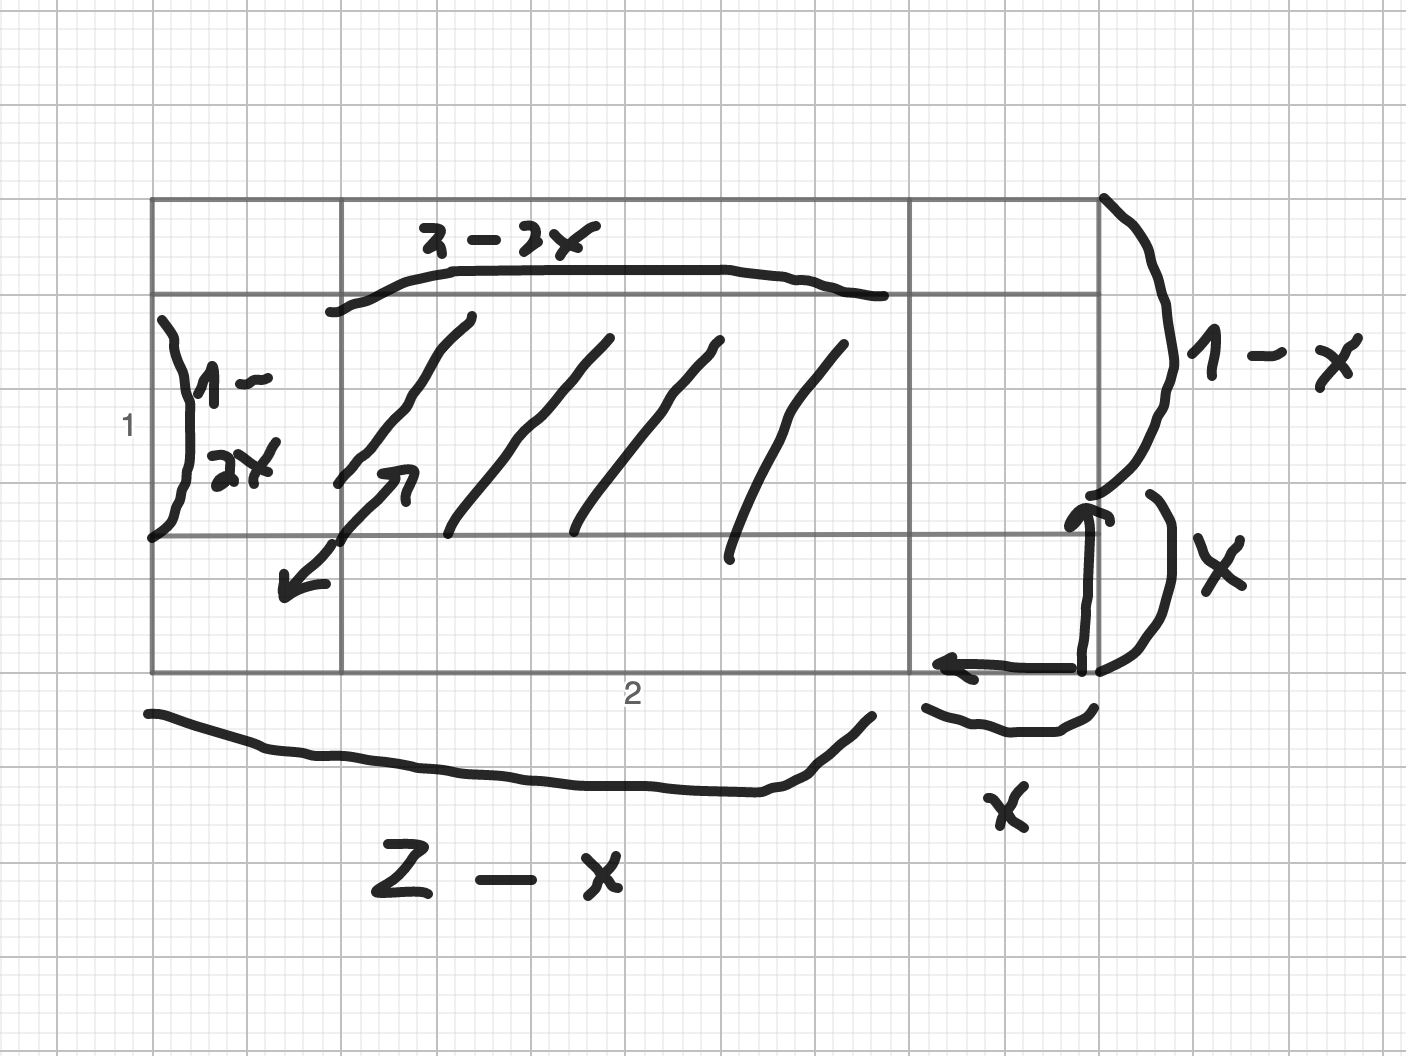
\includegraphics[scale=0.3]{3.png}
\end{center}
Картина не оч красивая, но не суть.  От каждой стороны мы отошли на $x$ и получили прямоугольник с параметрическими сторонами $1 - 2x, 2-2x$, которые зависят соотвественно от $x$. Он может увеличиваться и уменьшаться в размере по стрелочке соотвественно, но т.к $x < \frac12$, там всегда будет какая-то площадь. Именно в этой площади будут точки, которые на расстоянии больше $x$, они нам не подходят, т.е:
\[
P(A) = 1 - P(\text{точка лежит внутри прямоугольника})
\]
Найдем эту вероятность:
\[
P(\text{точка лежит внутри прямоугольника}) = \frac{S\text{(подходит нам)}}{S(\text{общая)}} = \frac{(2-2x)(1-2x)}{2 \cdot 1} =
\]
\[
 = 2x^2 - 3x + 1
\]
Тогда \textbf{ответ}:
\[
P(A) = 1 - (2x^2 - 3x +1 ) = 3x - 2x^2
\]
\end{itemize}
\subsection*{b) [до каждой стороны]}
Разобьем на случаи:
\begin{itemize}
\item $0 < x \leq 1$:

Очевидно, что при таком $x$ у нас до хотя бы одной из сторон расстояние для любой точки будет больше $x$, т.к у нас прямоугольник 2 на 1, т.е $P(A) = 0$
\item $1 < x < 2$:
При таком $x$ расстояние до верхней и нижней прямой не будет превосходить $x$ (т.к сверху вниз у нас высота 1). А вот для левой и правой стороны нужно ограничить параметрическую фигуру, отойдя слева и справа на $x$ соотвественно, т.е:
\begin{center}
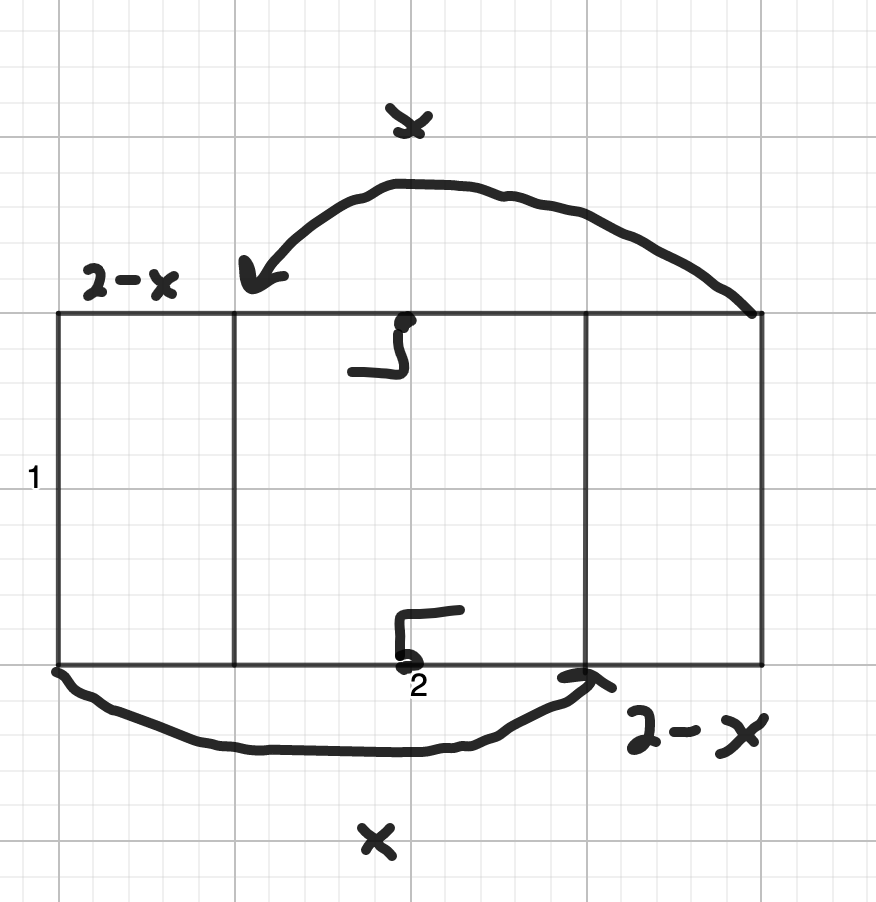
\includegraphics[scale=0.3]{4.png}
\end{center}
Чтобы точка была не больше $x$ до каждой из сторон, она должна быть внутри центрального прямоугольника, ибо если она будет слева или справа, то до правой(левой соответственно) стороны будет расстояние $>x$ и этот случай нам подходить не будет, итого:
\[
P(A) = \frac{1 \cdot (2 - 2(2-x))}{2} = \frac{2 - 4 + 2x}{2} = 1 - 2 + x = x - 1
\]
\item $x \geq 2$:
Очевидно, что расстояние никак не может быть больше 2, поэтому тут всегда $P(A) = 1$
\end{itemize} 
\end{document}
